\section{Assignment \#2}

% begin subsection
\subsection{Write a C program to find maximum between two numbers.}
\textbf{Program Code}
\inputminted[breaklines]{C}{programs/A02_P01.c}
\textbf{Program Output}
\begin{figure}[h]
  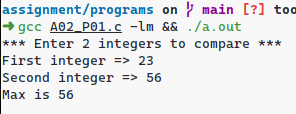
\includegraphics[width=10cm]{A02_P01}
\end{figure}
\pagebreak
% end subsection

% begin subsection
\subsection{Write a C program to find maximum between three numbers.}
\textbf{Program Code}
\inputminted[breaklines]{C}{programs/A02_P02.c}
\textbf{Program Output}
\begin{figure}[h]
  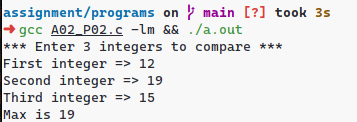
\includegraphics[width=10cm]{A02_P02}
\end{figure}
\pagebreak
% end subsection

% begin subsection
\subsection{Write a C program to check whether a number is negative, positive or zero.}
\textbf{Program Code}
\inputminted[breaklines]{C}{programs/A02_P03.c}
\textbf{Program Output}
\begin{figure}[h]
  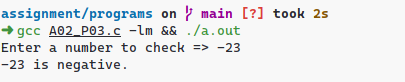
\includegraphics[width=10cm]{A02_P03}
\end{figure}
\pagebreak
% end subsection

% begin subsection
\subsection{Write a C program to check whether a number is divisible by 5 and 11 or not.}
\textbf{Program Code}
\inputminted[breaklines]{C}{programs/A02_P04.c}
\textbf{Program Output}
\begin{figure}[h]
  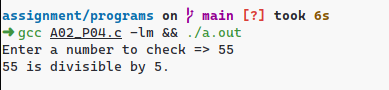
\includegraphics[width=10cm]{A02_P04}
\end{figure}
\pagebreak
% end subsection

% begin subsection
\subsection{Write a C program to check whether a number is even or odd.}
\textbf{Program Code}
\inputminted[breaklines]{C}{programs/A02_P05.c}
\textbf{Program Output}
\begin{figure}[h]
  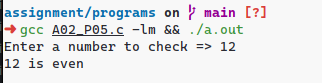
\includegraphics[width=10cm]{A02_P05}
\end{figure}
\pagebreak
% end subsection

% begin subsection
\subsection{[FIXME] Write a C program to check whether a year is leap year or not.}
\textbf{Program Code}
\inputminted[breaklines]{C}{programs/A02_P06.c}
\textbf{Program Output}
\begin{figure}[h]
  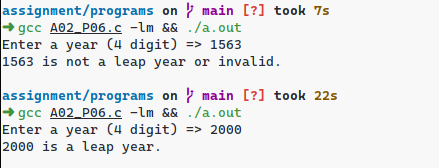
\includegraphics[width=10cm]{A02_P06}
\end{figure}
\pagebreak
% end subsection


% begin subsection
\subsection{Write a C program to check whether a character is alphabet or not.}
\textbf{Program Code}
\inputminted[breaklines]{C}{programs/A02_P07.c}
\textbf{Program Output}
\begin{figure}[h]
  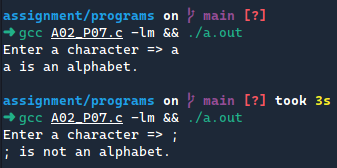
\includegraphics[width=10cm]{A02_P07}
\end{figure}
\pagebreak
% end subsection

% begin subsection
\subsection{Write a C program to input any alphabet and check whether it is vowel or consonant.}
\textbf{Program Code}
\inputminted[breaklines]{C}{programs/A02_P08.c}
\textbf{Program Output}
\begin{figure}[h]
  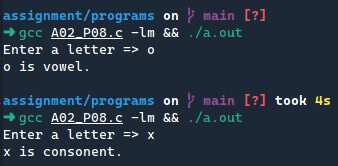
\includegraphics[width=10cm]{A02_P08}
\end{figure}
\pagebreak
% end subsection

% begin subsection
\subsection{Write a C program to input any character and check whether it is alphabet, digit or special character.}
\textbf{Program Code}
\inputminted[breaklines]{C}{programs/A02_P09.c}
\textbf{Program Output}
\begin{figure}[h]
  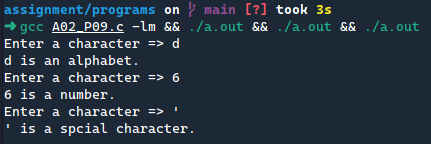
\includegraphics[width=10cm]{A02_P09}
\end{figure}
\pagebreak
% end subsection

% begin subsection
\subsection{Write a C program to check whether a character is uppercase or lowercase alphabet.}
\textbf{Program Code}
\inputminted[breaklines]{C}{programs/A02_P10.c}
\textbf{Program Output}
\begin{figure}[h]
  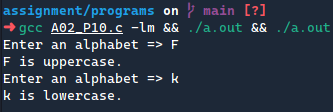
\includegraphics[width=10cm]{A02_P10}
\end{figure}
\pagebreak
% end subsection

% begin subsection
\subsection{Write a C program to input week number and print week day.}
\textbf{Program Code}
\inputminted[breaklines]{C}{programs/A02_P11.c}
\textbf{Program Output}
\begin{figure}[h]
  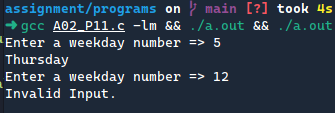
\includegraphics[width=10cm]{A02_P11}
\end{figure}
\pagebreak
% end subsection

% begin subsection
\subsection{Write a C program to input month number and print number of days in that month.}
\textbf{Program Code}
\inputminted[breaklines]{C}{programs/A02_P12.c}
\textbf{Program Output}
\begin{figure}[h]
  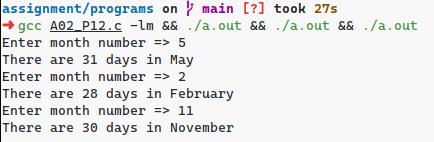
\includegraphics[width=10cm]{A02_P12}
\end{figure}
\pagebreak
% end subsection

% begin subsection
\subsection{Write a C program to count total number of notes in given amount.}
\textbf{Program Code}
\inputminted[breaklines]{C}{programs/A02_P13.c}
\textbf{Program Output}
\begin{figure}[h]
  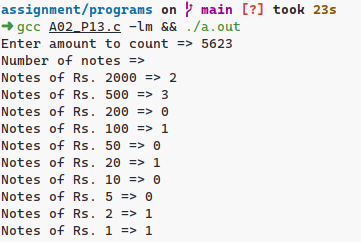
\includegraphics[width=10cm]{A02_P13}
\end{figure}
\pagebreak
% end subsection

% begin subsection
\subsection{Write a C program to input angles of a triangle and check whether triangle is valid or not.}
\textbf{Program Code}
\inputminted[breaklines]{C}{programs/A02_P14.c}
\textbf{Program Output}
\begin{figure}[h]
  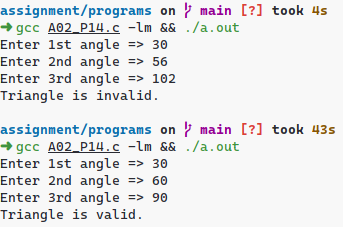
\includegraphics[width=10cm]{A02_P14}
\end{figure}
\pagebreak
% end subsection

% begin subsection
\subsection{Write a C program to input all sides of a triangle and check whether triangle is valid or not.}
\textbf{Program Code}
\inputminted[breaklines]{C}{programs/A02_P15.c}
\textbf{Program Output}
\begin{figure}[h]
  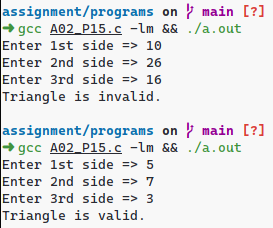
\includegraphics[width=10cm]{A02_P15}
\end{figure}
\pagebreak
% end subsection

% begin subsection
\subsection{Write a C program to check whether the triangle is equilateral, isosceles or scalene triangle.}
\textbf{Program Code}
\inputminted[breaklines]{C}{programs/A02_P16.c}
\textbf{Program Output}
\begin{figure}[h]
  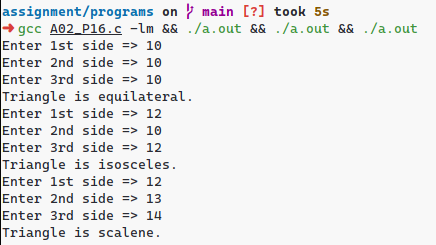
\includegraphics[width=10cm]{A02_P16}
\end{figure}
\pagebreak
% end subsection

% begin subsection
\subsection{[TODO] Write a C program to find all roots of a quadratic equation.}
\textbf{Program Code}
\inputminted[breaklines]{C}{programs/A02_P17.c}
\textbf{Program Output}
\begin{figure}[h]
  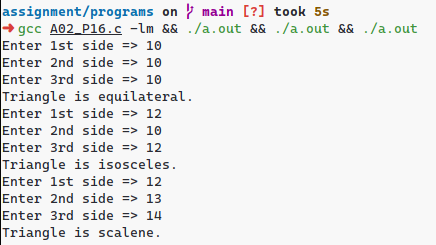
\includegraphics[width=10cm]{A02_P16}
\end{figure}
\pagebreak
% end subsection

% begin subsection
\subsection{Write a C program to calculate profit or loss.}
\textbf{Program Code}
\inputminted[breaklines]{C}{programs/A02_P18.c}
\textbf{Program Output}
\begin{figure}[h]
  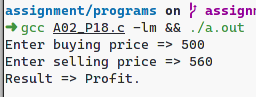
\includegraphics[width=10cm]{A02_P18}
\end{figure}
\pagebreak
% end subsection

% begin subsection
\subsection{Write a C program to input marks of five subjects Physics, Chemistry, Biology, Mathematics and Computer. Calculate percentage and grade according to following.}
\begin{itemize}
  \item $Percentage \geq 90\% : Grade A$
  \item $Percentage \geq 80\% : Grade B$
  \item $Percentage \geq 70\% : Grade C$
  \item $Percentage \geq 60\% : Grade D$
  \item $Percentage \geq 40\% : Grade E$
  \item $Percentage < 40\% : Grade F$
\end{itemize}


\textbf{Program Code}
\inputminted[breaklines]{C}{programs/A02_P19.c}
\textbf{Program Output}
\begin{figure}[h]
  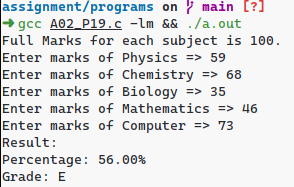
\includegraphics[width=10cm]{A02_P19}
\end{figure}
\pagebreak
% end subsection

% begin subsection
\subsection{[TODO] Write a C program to input basic salary of an employee and calculate its Gross salary according to following.}
\begin{itemize}
  \item $Basic Salary <= 10000 : HRA = 20\%, DA = 80\%$
  \item $Basic Salary <= 20000 : HRA = 25\%, DA = 90\%$
  \item $Basic Salary > 20000 : HRA = 30\%, DA = 95\%$
\end{itemize}
\textbf{Program Code}
\inputminted[breaklines]{C}{programs/A02_P19.c}
\textbf{Program Output}
\begin{figure}[h]
  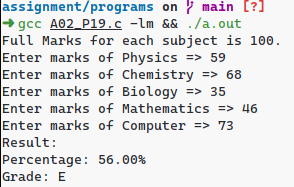
\includegraphics[width=10cm]{A02_P19}
\end{figure}
\pagebreak
% end subsection


% begin subsection
\subsection{Write a C program to input electricity unit charges and calculate total electricity bill according to the given condition.}
\begin{itemize}
  \item For first 50 units Rs. 0.50/unit
  \item For next 100 units Rs. 0.75/unit
  \item For next 100 units Rs. 1.20/unit
  \item For unit above 250 Rs. 1.50/unit
  \item An additional surcharge of 20\% is added to the bill
\end{itemize}
\textbf{Program Code}
\inputminted[breaklines]{C}{programs/A02_P21.c}
\textbf{Program Output}
\begin{figure}[h]
  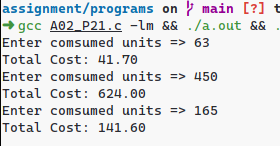
\includegraphics[width=10cm]{A02_P21}
\end{figure}
\pagebreak
% end subsection
